\documentclass[a4paper, 12pt]{article}

%%% SST LAB PROTOCOLL PREAMBLE
%%% 2019
%%%%%%%%%%%%%%%%%%%%%%%%%%%%%%%


%%% PACKAGES
%%%%%%%%%%%%%%%%%%%%%%%%%%%

\usepackage[ngerman]{babel}

\usepackage[utf8]{inputenc}
\usepackage{amsmath}
\usepackage{pgfplots}
\usepackage{tikz}
\usepackage[many]{tcolorbox}
\usepackage{graphicx}
\graphicspath{ {./graphics/} }
\usepackage{pdfpages}
\usepackage{dashrule}
\usepackage{float}
\usepackage{siunitx}
\usepackage{trfsigns}
\usepackage{booktabs}
\usepackage[european]{circuitikz}
\usepackage{tcolorbox}

%%% DOCUMENT GEOMETRY
%%%%%%%%%%%%%%%%%%%%%%%%%%%

\usepackage{geometry}
\geometry{
 a4paper,
 total={0.6180339887498948\paperwidth,0.6180339887498948\paperheight},
 top = 0.1458980337503154\paperheight,
 bottom = 0.1458980337503154\paperheight
 }
\setlength{\jot}{0.013155617496424828\paperheight}
\linespread{1.1458980337503154}

\setlength{\parskip}{0.013155617496424828\paperheight} % paragraph spacing


%%% COLORS
%%%%%%%%%%%%%%%%%%%%%%%%%%%

\definecolor{red1}{HTML}{f38181}
\definecolor{yellow1}{HTML}{fce38a}
\definecolor{green1}{HTML}{95e1d3}
\definecolor{blue1}{HTML}{66bfbf}
\definecolor{hsblue}{HTML}{00b1db}
\definecolor{hsgrey}{HTML}{afafaf}

%%% CONSTANTS
%%%%%%%%%%%%%%%%%%%%%%%%%%%
\newlength{\smallvert}
\setlength{\smallvert}{0.0131556\paperheight}


%%% COMMANDS
%%%%%%%%%%%%%%%%%%%%%%%%%%%

% differential d
\newcommand*\dif{\mathop{}\!\mathrm{d}}

% horizontal line
\newcommand{\holine}[1]{
  	\begin{center}
	  	\noindent{\color{hsgrey}\hdashrule[0ex]{#1}{1pt}{3mm}}\\%[0.0131556\paperheight]
  	\end{center}
}

% mini section
\newcommand{\minisec}[1]{ \noindent\underline{\textit {#1} } \\}

% quick function plot
\newcommand{\plotfun}[3]{
  \vspace{0.021286\paperheight}
  \begin{center}
    \begin{tikzpicture}
      \begin{axis}[
        axis x line=center,
        axis y line=center,
        ]
        \addplot[draw=red1][domain=#2:#3]{#1};
      \end{axis}
    \end{tikzpicture}
  \end{center}
}

% box for notes
\newcommand{\notebox}[1]{

\tcbset{colback=white,colframe=green1!100!black,title=Note!,width=0.618\paperwidth,arc=0pt}

 \begin{center}
  \begin{tcolorbox}[]
   #1 
  \end{tcolorbox}
 
 \end{center} 
 
}

% box for equation
\newcommand{\eqbox}[2]{
	
	\tcbset{colback=white,colframe=green1!100!black,title=,width=#2,arc=0pt}
	
	\begin{center}
		\begin{tcolorbox}[ams align*]
				#1
		\end{tcolorbox}
		
	\end{center} 
	
}
% END OF PREAMBLE

%%%%%%%%%%%%%%%%%%%%%%%%%%%%%%%%%%%%%

\begin{document}

%%%%%%%%%%%%%%%%%%%%%%%%%%%%%%%%%%%%%
  
\includepdf{./titlepage/titlepage.pdf}
  \clearpage
  \setcounter{page}{1}
%%%%%%%%%%%%%%%%%%%%%%%%%%%%%%%%%%%%%

  \section{Aufgabe 1: Digitale Modulation (1), Bandbreitenmessung}

  \begin{figure}[H]
    \begin{center}
      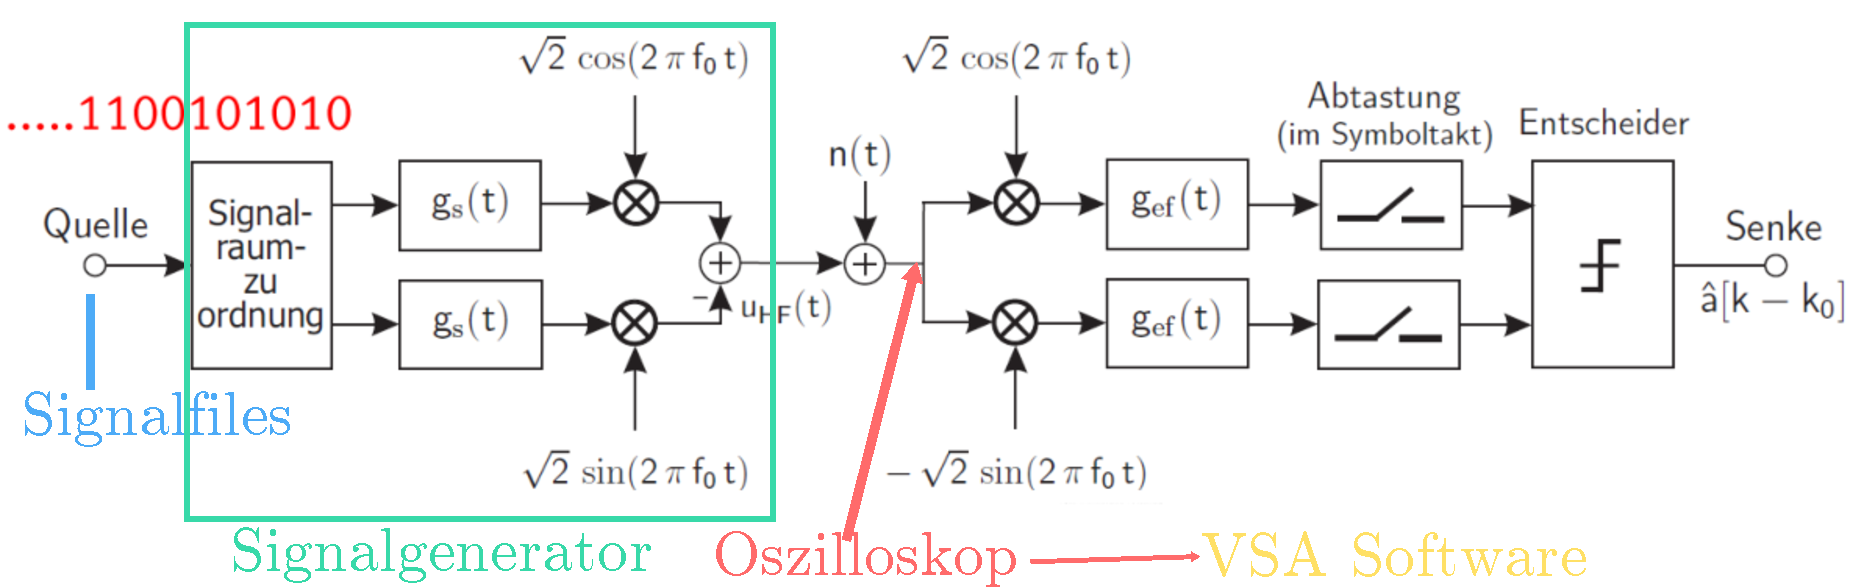
\includegraphics[width=\textwidth]{1/blockschaltbild.pdf}
    \end{center}
    \caption{Versuchsaufbau}
  \end{figure}
  Im Versuch sollten die Bandbreiten von drei QPSK-modulierten Signalen mit
  unterschiedlichen Symbolraten bestimmt und die Unterschiede zur
  Basisbandübertragung verdeutlicht werden.

  \subsection{Einstellungen}
  Der Signalgenerator wurde zuerst auf eine Trägerfrequenz von $2.4 \,
  \si{\giga\hertz}$ eingestellt und es wurden die im Speicher befindlichen
  Dateien der QPSK-Daten mit den entsprechenden Symbolraten ausgewählt. Zur korrekten
  Wiedergabe der Signaldateien musste außerdem 4-fach Oversampling ($4 \,
  \si{\mega\hertz}, 16 \, \si{\mega\hertz}, 32 \, \si{\mega\hertz} $) eingestellt werden. Die Sendeleistung wurde auf $1 \,
  \si{\milli\watt}$(Amplitude: $0 \, \si{\deci\bel}\textrm{m}$) gesetzt.

  \begin{figure}[H]
    \begin{center}
      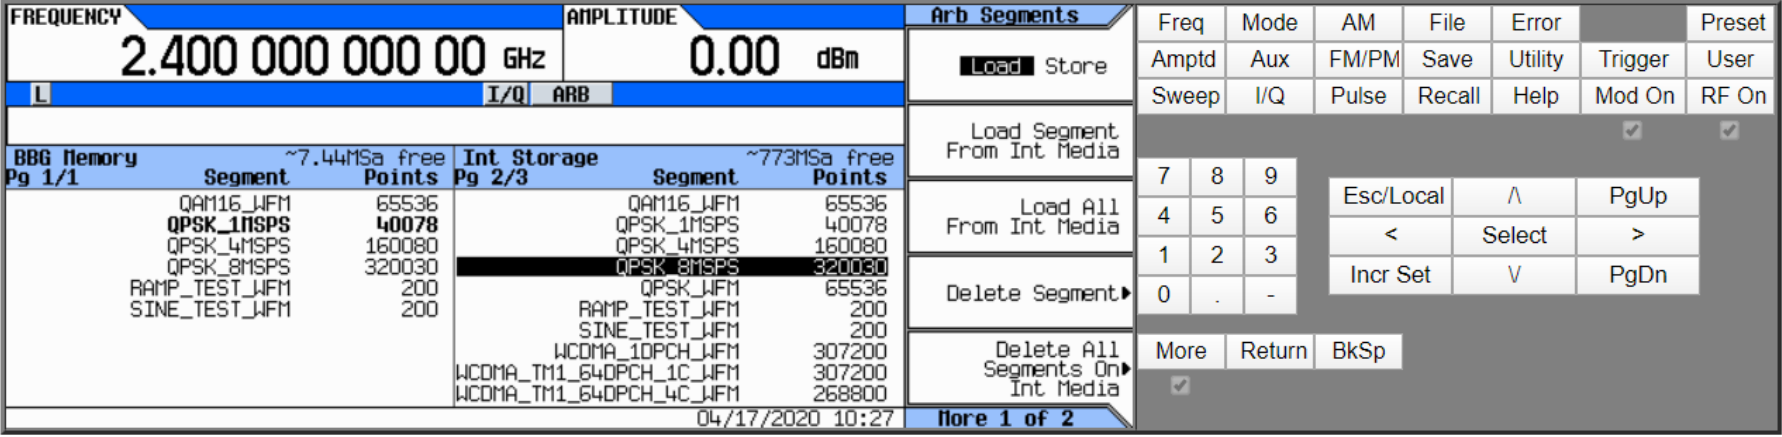
\includegraphics[width=\textwidth]{1/einstellung_transmitter}
    \end{center}
    \caption{Einstellungen am Signalgenerator (N5182A)}
  \end{figure}


  \subsection{Messung}

  Zunächst wurde das Zeitsignal am Oszillsokop (Abb. 3) dargestellt. 
  Mithilfe der FFT-Funktion wurde dann das Spektrum eines Signals ermittelt.
Zur erfolgreichen Darstellung des
  Spektrums bei einem Span von $20 \, \si{\mega\hertz}$ wurde die Auflösungsbandbreite
  (Resolution Bandwidth, RBW) auf $30 \, \si{\kilo\hertz}$ verringert. 
  Abbildung 4 zeigt das Empfangssignal mit einer anderen Zeitauflösung, welche
  durch die FFT eingestellt wurde. Hieran lässt sich ein typischer Signalverlauf
  eines digitalmodulierten Signals erkennen. 

  \begin{figure}[H]
    \begin{center}
      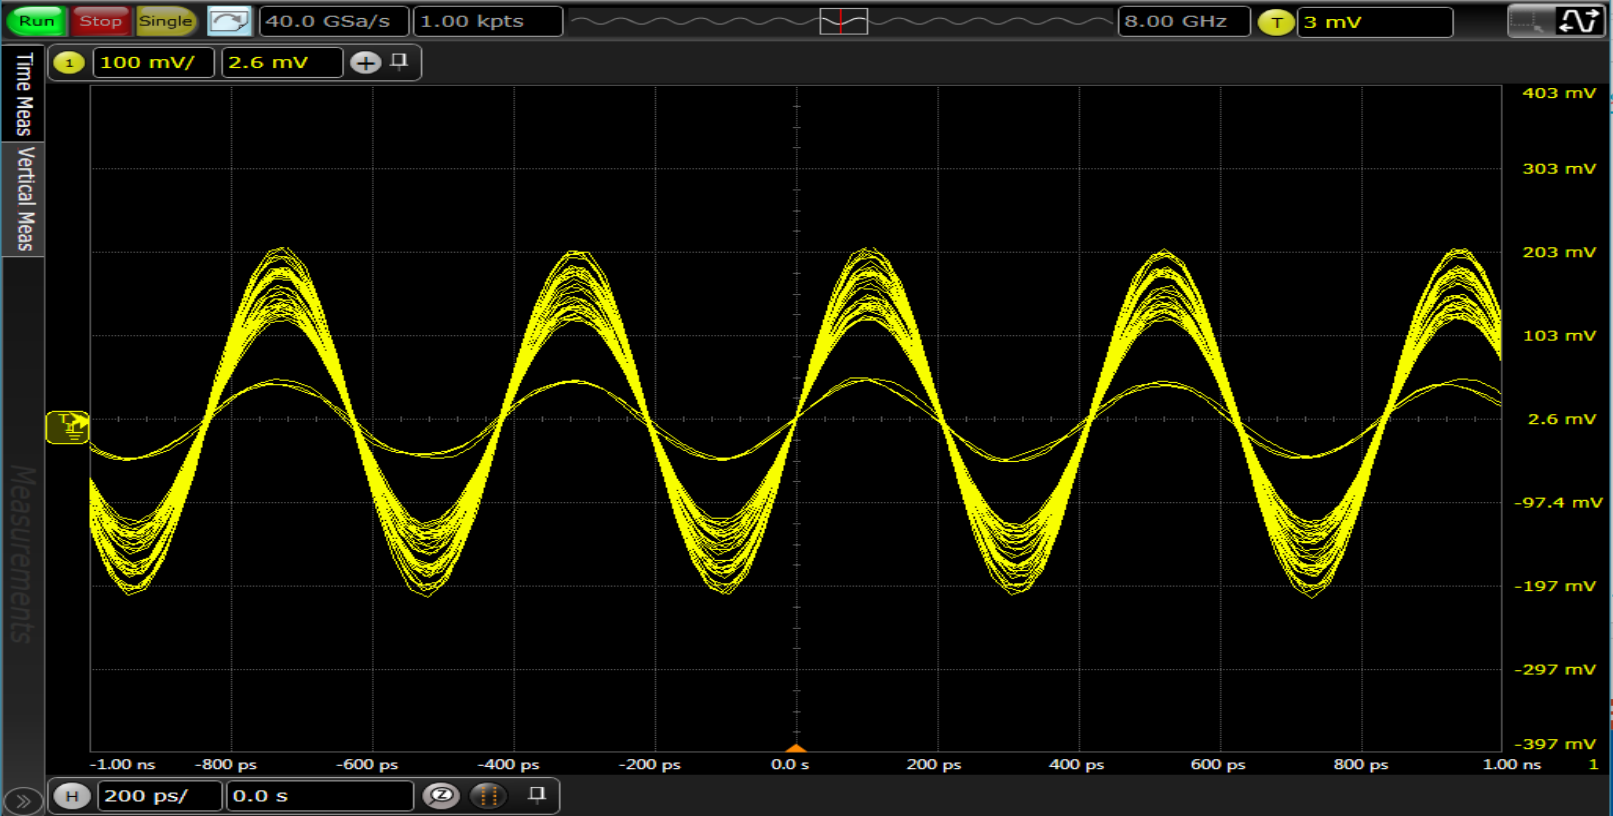
\includegraphics[width=\textwidth]{1/oszi_zeitsignal}
    \end{center}
    \caption{QPSK-Zeitsignal am Oszilloskop}
  \end{figure}

  \begin{figure}[H]
    \begin{center}
      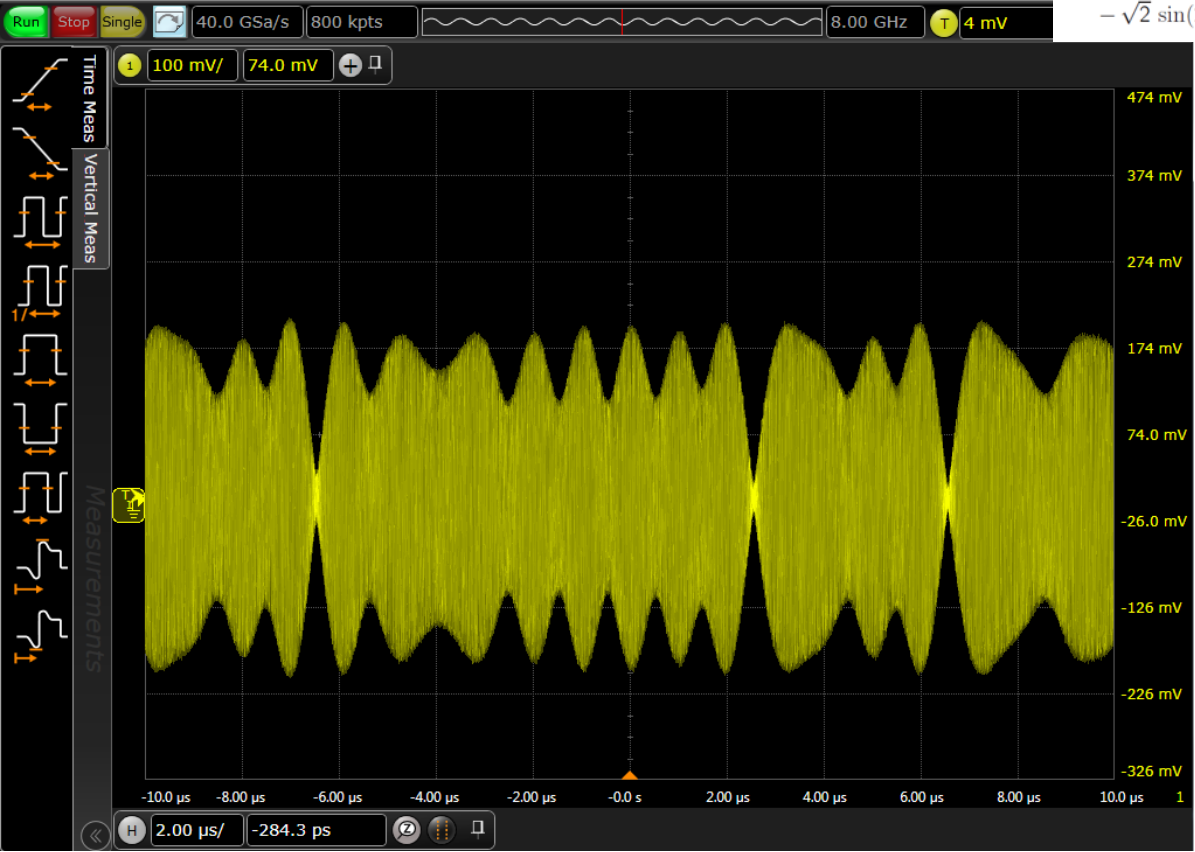
\includegraphics[width=\textwidth]{1/oszi_zeitsignal2}
    \end{center}
    \caption{QPSK-Zeitsignal am Oszilloskop, andere Zeitauflösung}
  \end{figure}

  Um die Signale detaillierter analysieren zu können, wurden die aufgenommenen
  Oszilloskopdaten in die VSA-Software gegeben, in welcher dann Spektrum und
  Occupied Bandwidth (OBW) ermittelt wurden, Abb. 5, Abb. 6 und Abb. 7 zeigen
  Screenshots der VSA Oberfläche bei den einzelnen Symbolraten. Das obere
  Fenster zeigt das jeweilige Spektrum, das untere den Verlauf der Realen
  Komponente des Zeitsignals.
  
    \begin{figure}[H]
    \begin{center}
      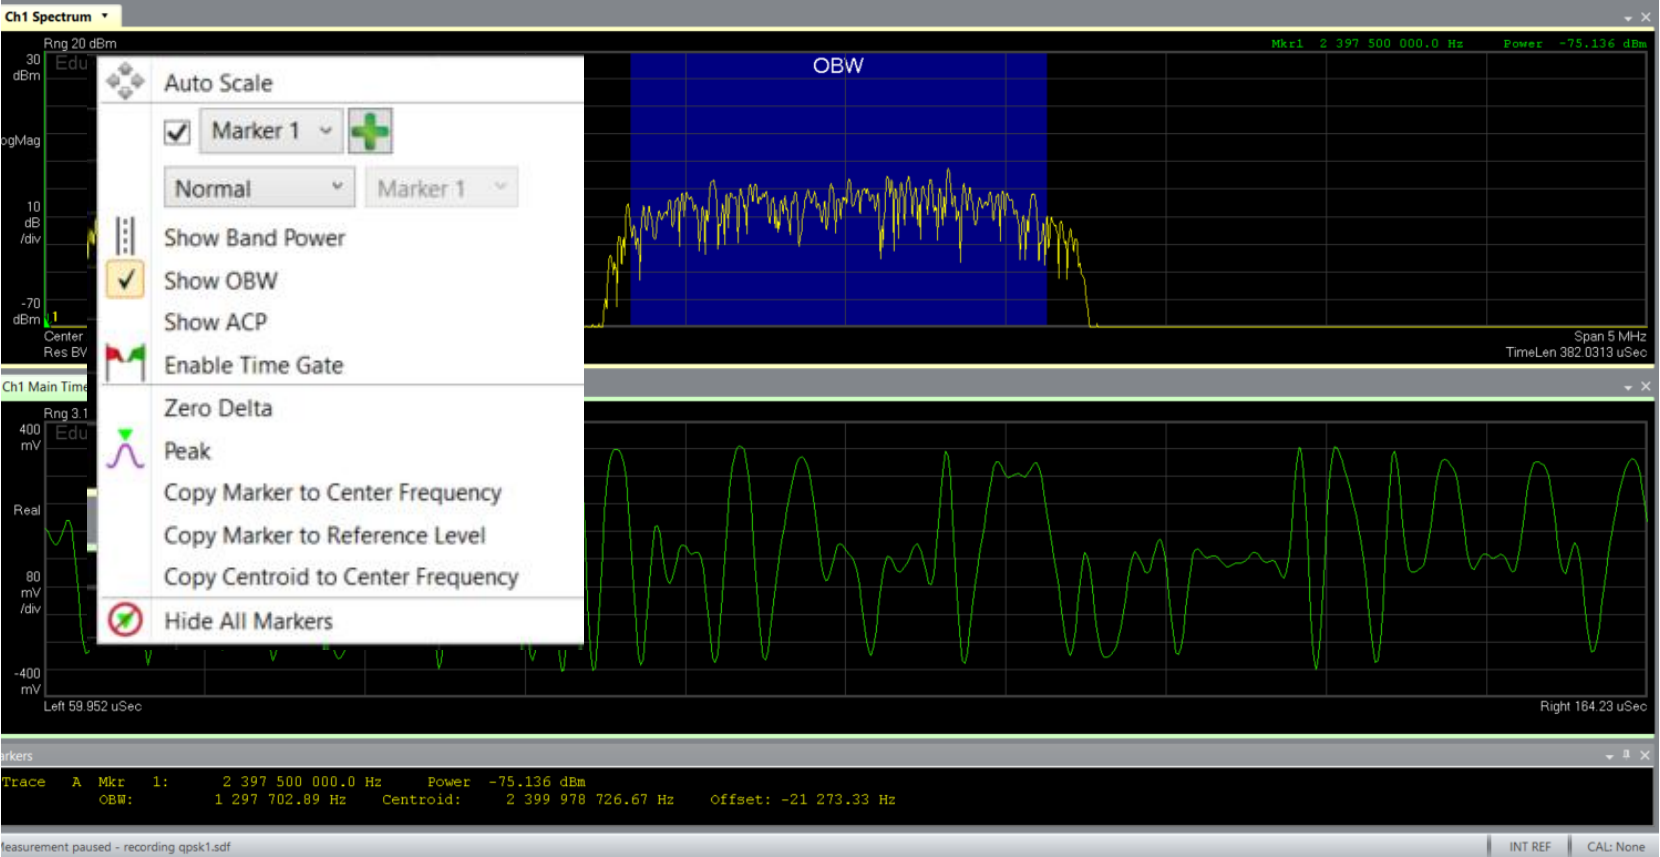
\includegraphics[width=\textwidth]{1/QPSK1}
    \end{center}
    \caption{VSA bei $f_T = 1 \, \si{MSps}$}
  \end{figure}
    \begin{figure}[H]
    \begin{center}
      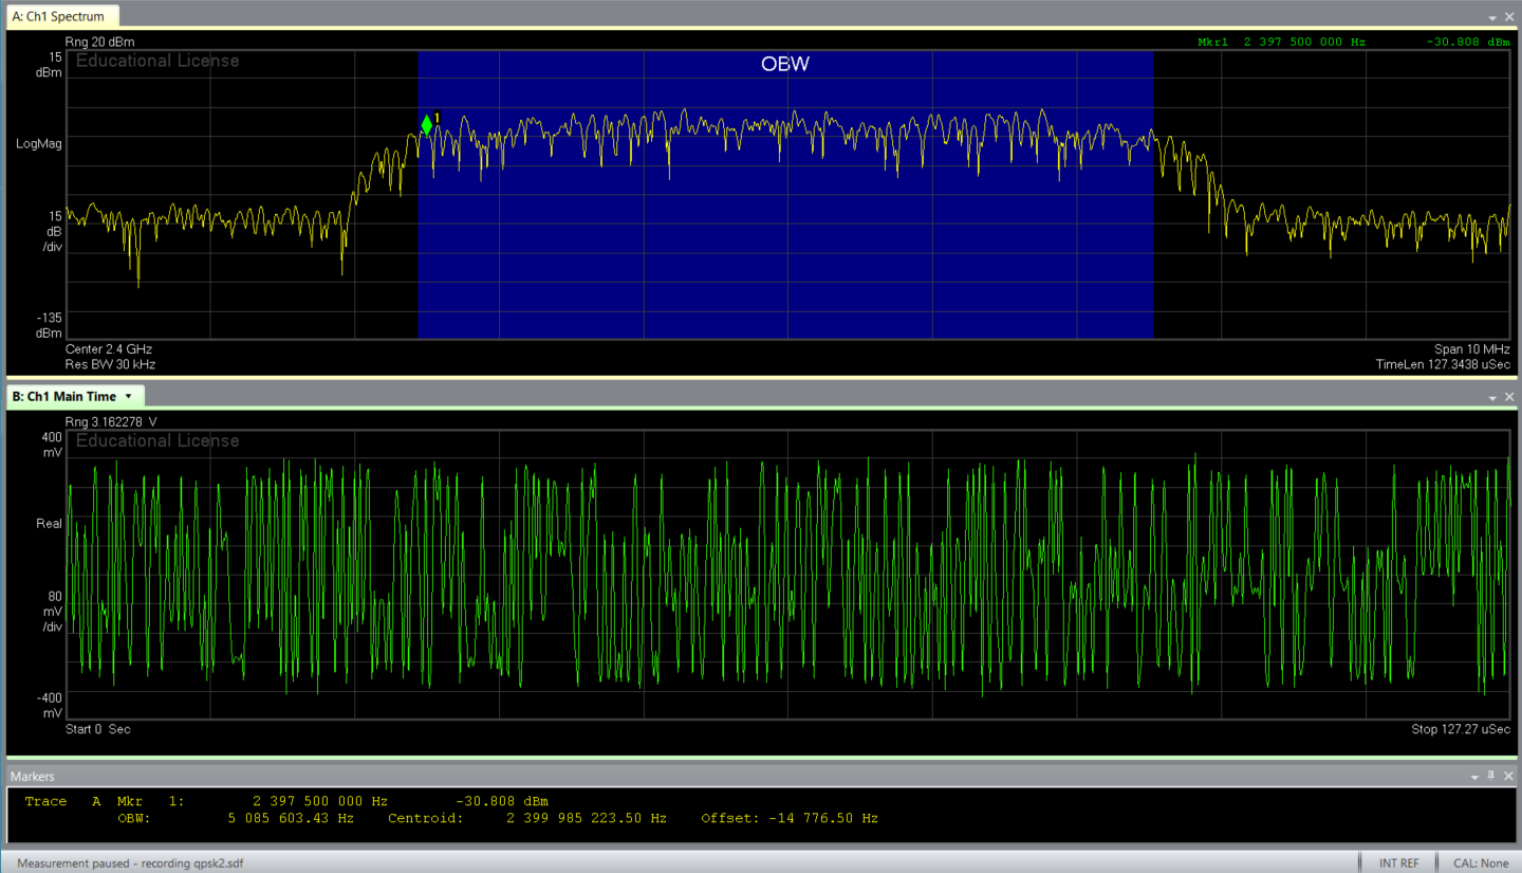
\includegraphics[width=\textwidth]{1/QPSK2}
    \end{center}
    \caption{VSA bei $f_T = 4 \, \si{MSps}$}
  \end{figure}
    \begin{figure}[H]
    \begin{center}
      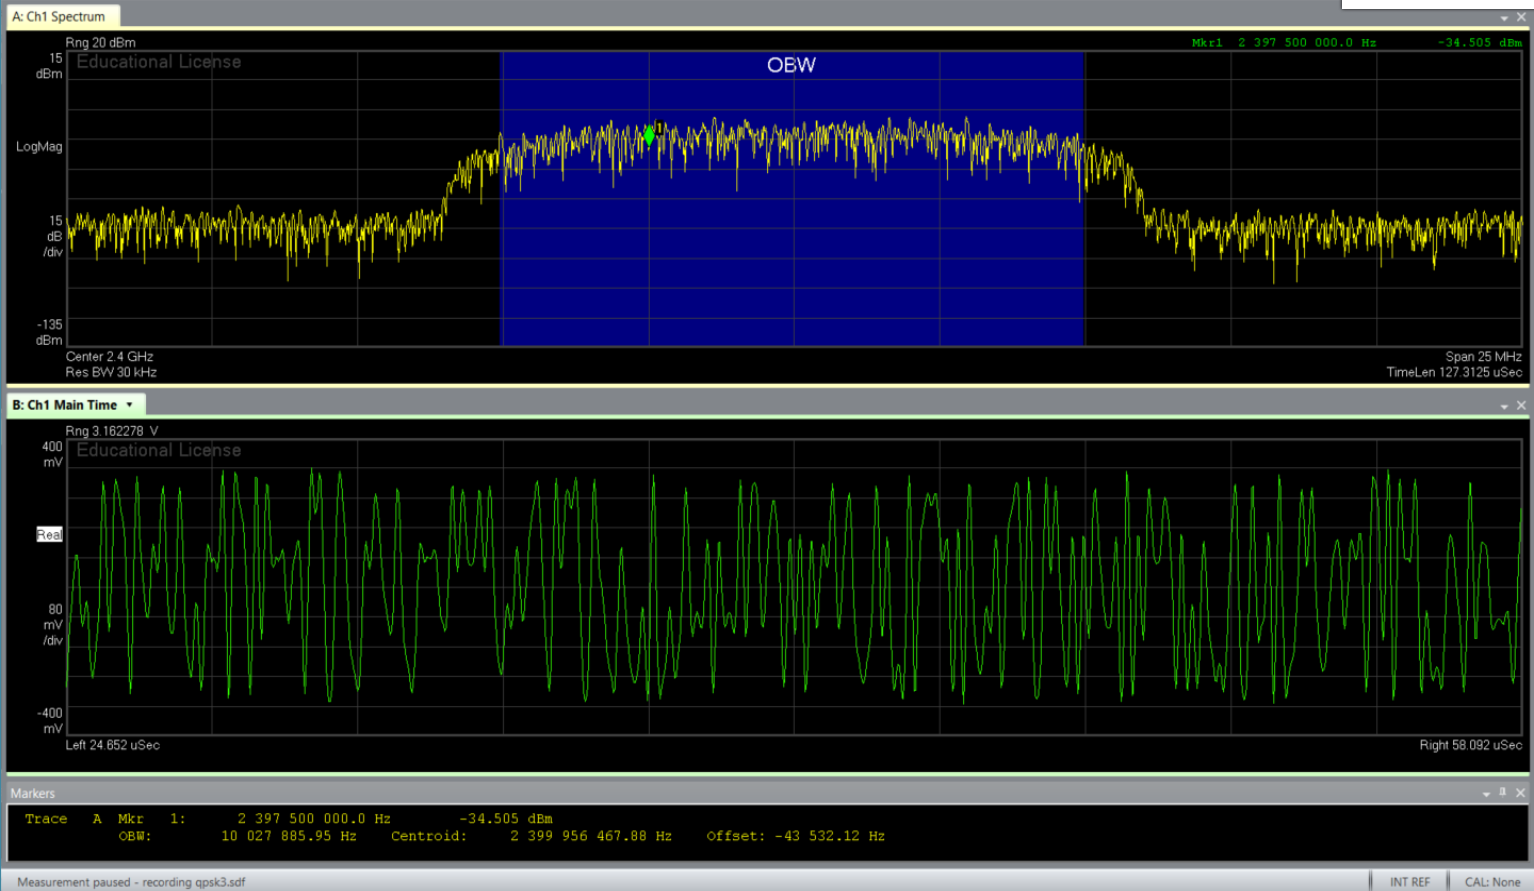
\includegraphics[width=\textwidth]{1/QPSK3}
    \end{center}
    \caption{VSA bei $f_t = 8 \, \si{MSps}$}
  \end{figure}

Die Ergebnisse der Messung sind in Tabelle 1 zu sehen.
  Die Bitrate bei der QPSK ist die doppelte Symbolrate, da zwei Bits je Symbol übertragen werden. 


  \begin{table}[H]
  \begin{center}
    \begin{tabular}{c | c }
      Symbolrate $f_T$ & Bandbreite $B$\\
      \hline
      $1 \, \textrm{MSps}$ & $1.298 \, \si{\mega\hertz}$\\
      $4 \, \textrm{MSps}$ & $5.086 \, \si{\mega\hertz}$\\
      $8 \, \textrm{MSps}$ & $10.028 \, \si{\mega\hertz}$
    \end{tabular}
    \caption{Messergebnisse der Aufgabe 1 (gerundet)}
  \end{center}
  \end{table}

  Trägt man die Werte in ein Digramm lässt sich ein linearer Zusammenhang
  zwischen Symbolrate und Bandbreite feststellen (Abb. 8).

  \begin{figure}[H]
    \begin{center}
      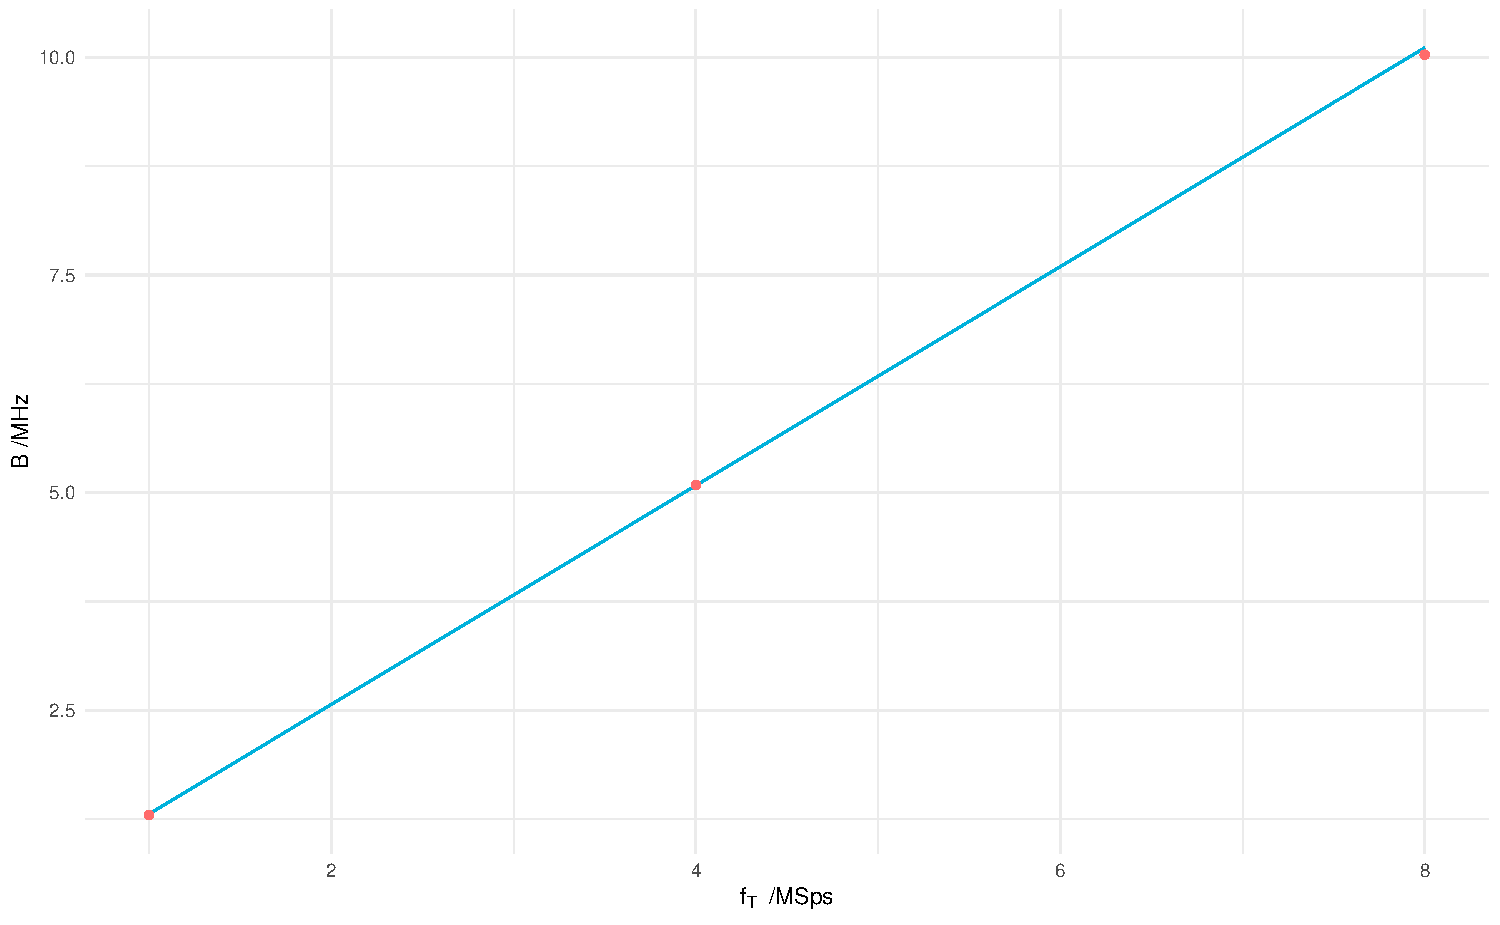
\includegraphics[width=\textwidth]{1/1_plot.pdf}
    \end{center}
    \caption{Messpunkte der Aufgabe 1 mit Regressionsgerade}
  \end{figure}

  \noindent Die lineare Regression der Messwerte liefert folgende Gleichung
  \begin{equation}
    B(f_T) = 1.24651 \frac{\si{\hertz}}{\si{Sps}} \cdot f_T + 0.06911 \, \si{\hertz}
    \end{equation}
  Die Bandbreite ist also etwa $25 \%$ größer als die Symbolrate.

 % Die theoretische Betrachtung liefert jedoch ein anderes Ergebnis. Die
 % Bandbreite eines Rechtecksignals nach der Impulsformung ist etwa
 % $\frac{1}{T}$, wobei $T$ die Impulsdauer ist. 

  Das Spektrum des QPSK-Signals (Bandpassbereich) stimmt mit dem des
  Basisbandsignals überein, lediglich die Mittenfrequenz ist anders, wodurch die
  'negativen' Frequenzen fehlen und die Bandbreite des Basisbandsignals
  gegenüber dem Bandpasssignal halbiert wird.

  
  
  \section{Aufgabe 2: Demodulation}

  Die VSA bietet eine digitale Demodulationsfunktion, welche im Praktikum verwendet
  wurde, um die Signale aus Aufgabe 1 zu demodulieren. Dabei musste darauf
  geachtet werden, dass Modulationsart und Symbolrate des Demodulators mit denen
  des Signals übereinstimmt, die Fehleinstellung ist in Abbildung 9 zu sehen.

  \begin{figure}[H]
    \begin{center}
      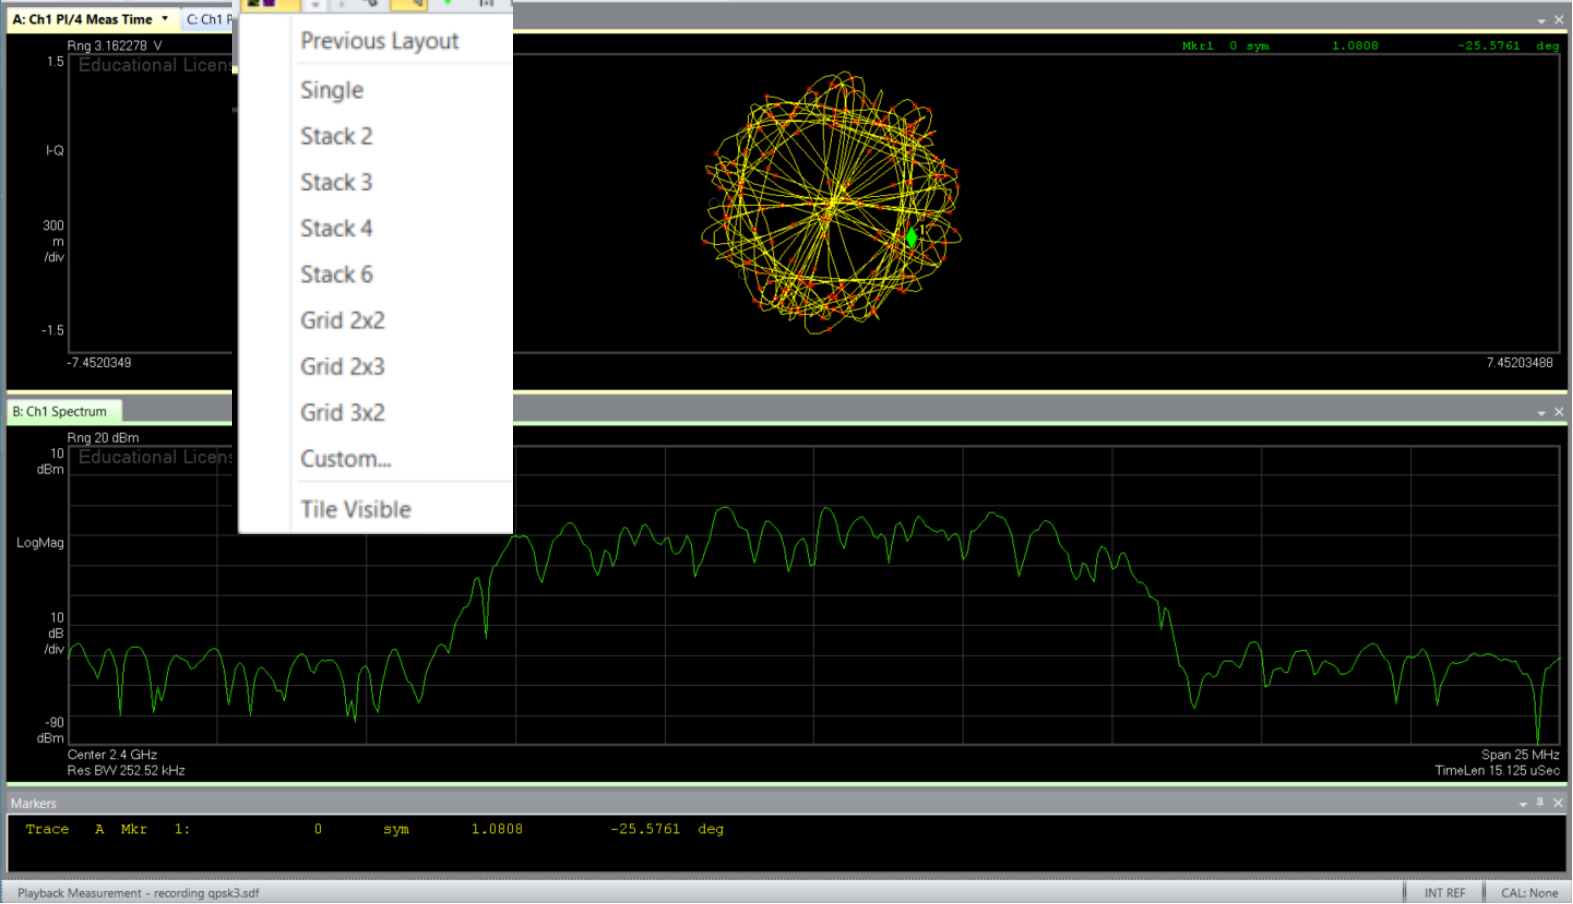
\includegraphics[width=\textwidth]{1/Demod_falsche_symrate}
    \end{center}
    \caption{Fehleinstellung der Demodulation}
  \end{figure}

  Für die Symbol-zu-Bit Zuordnung wurden Marker in der Signalraumdarstellung
  platziert, welche dann die entsprechenden Bits der Symbole angezeigt haben.
  In Abbildung 10 ist die Zuordnung zu erkennen, welche außerdem einer
  Gray-Codierung folgt. Dies ermöglicht, dass sich bei einem Symbolübergang
  maximal eine Bitstelle ändert (abgesehen von Diagonalübergängen). Weiterhin
  geschieht die Zuordnung der Symbole mit einer sehr geringen Streuung, was auf eine
  niedrige Fehlerrate der Entscheidung hinweist.

  \begin{figure}[H]
    \begin{center}
      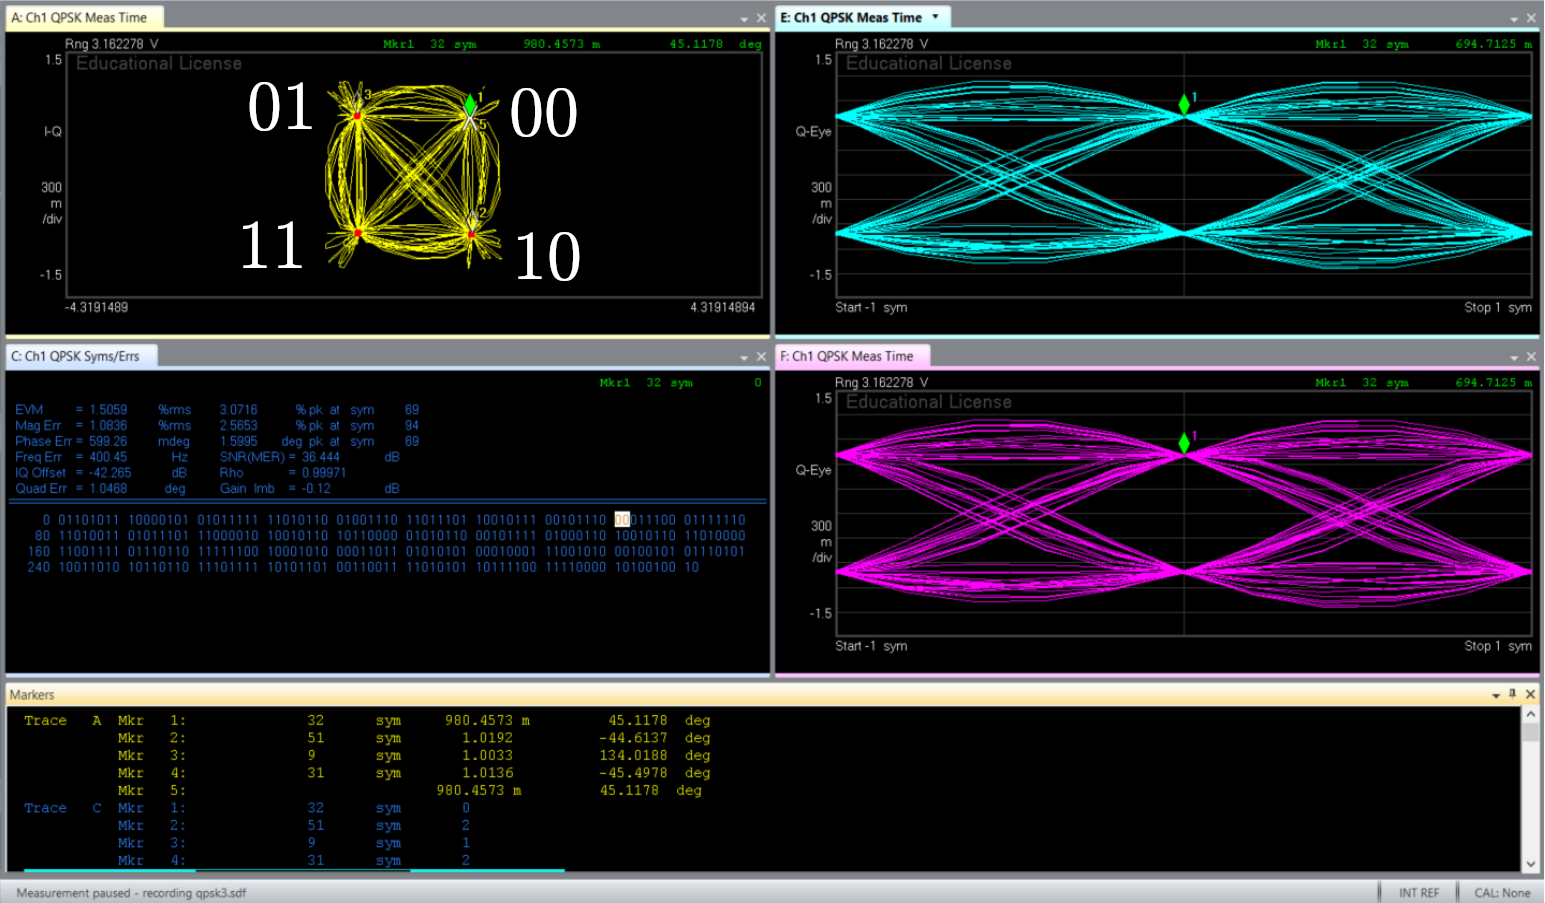
\includegraphics[width=\textwidth]{1/symzubit}
    \end{center}
    \caption{Symbol-zu-Bit-Dekodierung und Augendiagramme}
  \end{figure}

  Mithilfe des Augendiagrammes lässt sich u.a. die Erfüllung der ersten
  Nyquistbedingung überprüfen, welche fordert, dass vorhergehende und nachfolgende Impulse im
  Abtastzeitpunkt gleich null sein müssen. Das Augendiagramm stellt viele
  Zeitverläufe der Symboldauer $T$ des Detektionssignals übereinander dar, wodurch alle
  möglichen Signalübergänge und -zustände in
  einer Darstellung ersichtlich sind. In der Mitte der Zeitachse befindet sich
  der Zeitpunkt 0, i.e. der Abtastzeitpunkt, am rechten und linken Rand die
  Zeitpunkte $T$ bzw. $-T$.  Je kleiner die
  vertikale Augenöffnung, desto größer ist der Einfluss von Impulsinterferenzen,
  weshalb man generell an einer möglichst maximalen Augenöffnung interessiert ist.
  Die Augendiagramme aus Abbildung 10 gehören beide zur Q-Komponente des
  QPSK-Signals (Q-Eye). Man erkennt deutlich, dass im Abtastzeitpunkt keine
  Signalverläufe die Entscheidungsschwelle überschreiten, weshalb das erste
  Nyquistkriterium erfüllt ist.

  \section{Aufgabe 3: Digitale Modulation (2)}

  \begin{figure}[H]
    \begin{center}
      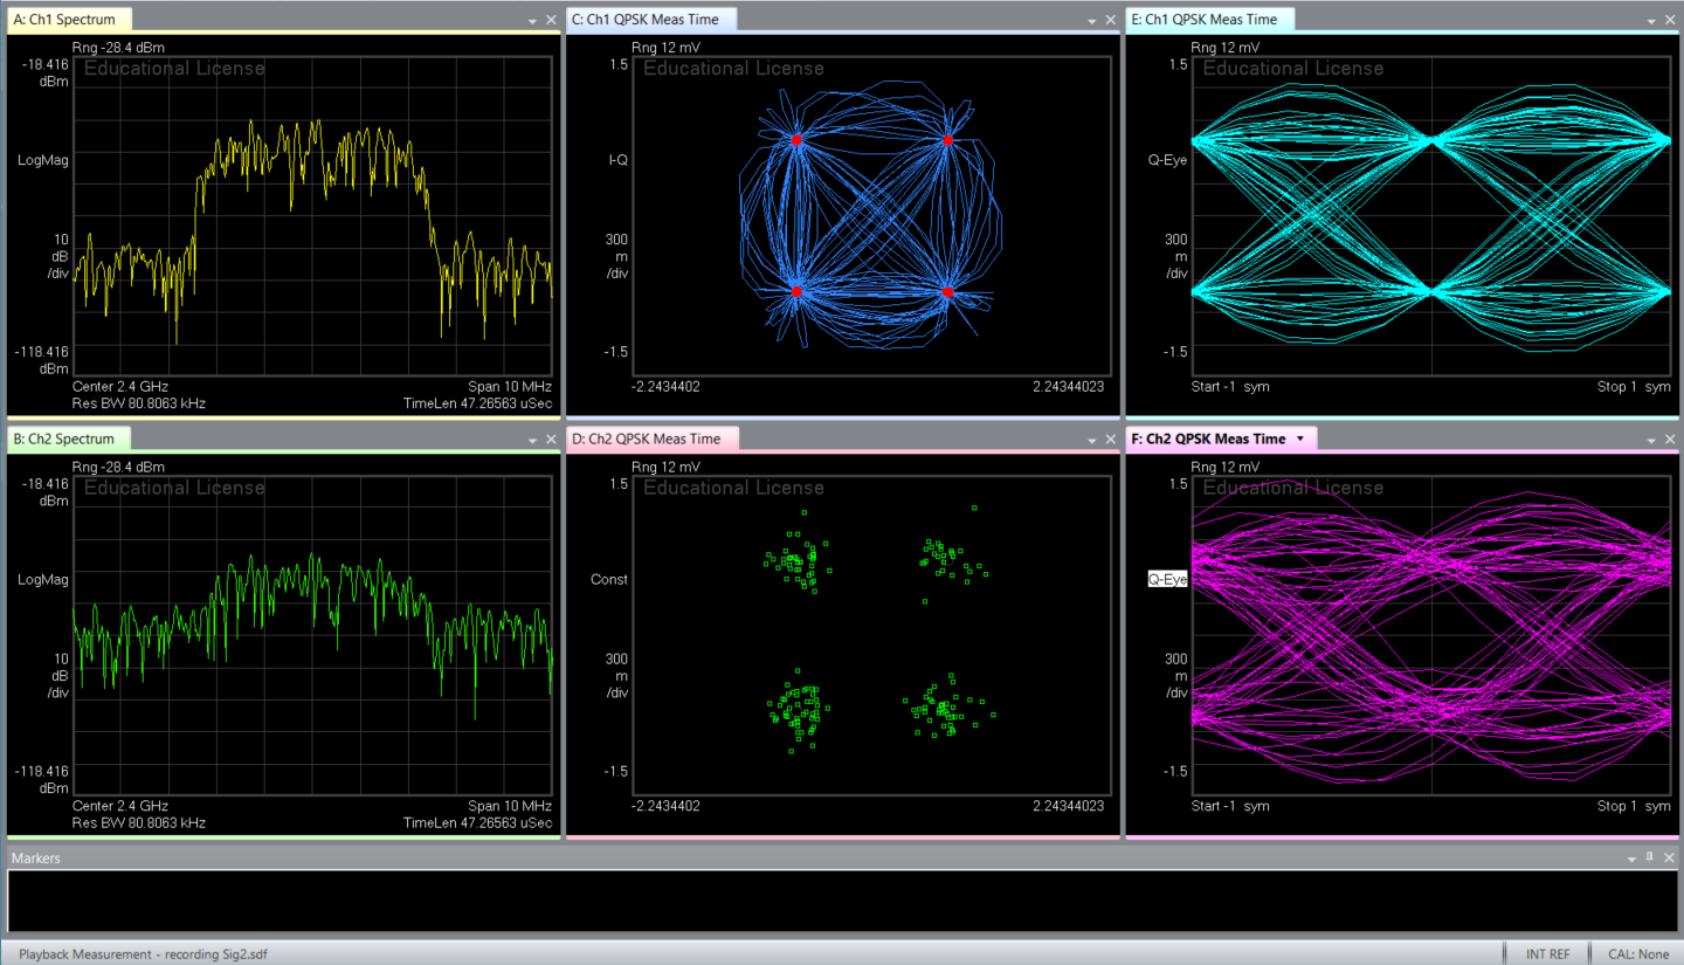
\includegraphics[width=\textwidth]{1/aufg3}
    \end{center}
    \caption{Messungen der Aufgabe 3}
  \end{figure}

  
  Die Spektren der Signale aus Abbildung 11 weisen beide ähnliche maximale
  Amplituden auf und belegen eine ähnliche Bandbreite, es lässt sich jedoch leicht
  erkennen, dass das Signal-Rausch-Verhältnis des unteren Signals geringer ist.
  Durch Schätzung der Bandbreite des oberen Signals und verwendung der Gleichung
  (1) aus der ersten Versuchsaufgabe kann die Symbolrate des Sendesignals
  ermittelt werden ($B \approx 4.5 \, \si{\mega\hertz}$).

  \[f_T \approx \frac{4.5 \, \si{\mega\hertz} - 0.06911 \, \si{\mega\hertz}}{1.24651
      \, \frac{\si{\mega\hertz}}{\si{MSps}}} \approx 3.56 \, \si{\mega Sps}\]

  Legt man die Entscheidungsschwelle an die Quadrantengrenzen bzw. I- und
  Q-Achsen, so treten Bitfehler auf sobald ein Konstellationspunkt diese
  überschreitet (z.B. 01 gesendet, 00 entschieden). Aus der zweiten Spalte von
  Abbildung 11 ist ersichtlich, dass die Punkte des Signals mit dem schlechteren
  SNR wesentlich stärker streuen, wodurch auch eine Fehlentscheidung
  wahrscheinlicher und die Bit-Error-Rate höher wird. Unter der Bedingung der
  Schwellen an den Quadrantengrenzen ist jedoch augenscheinlich nicht mit
  Bitfehlern zu rechnen. Allerdings verdeutlicht es auch die Störempfindlichkeit der
  Modulation, gerade bei einer höheren Anzahl an möglichen Symbolen und der damit
  höhreren Anzahl an Punkten im Konstellationsdiagramm, deren Schwellen deutlich näher beieinander liegen (wie z.B. bei QAM-16).

  Aus der (Q-)Augenöffnung des oberen Signals ist, wie in der vorherigen Aufgabe,
  eine ISI-freie Übertragung zu erkennen. Bei dem unteren Signal wird die
  Augenöffnung durch den stärkeren Rauscheinfluss verringert, die Signalverläufe
  liegen im Abtastzeitpunkt nicht mehr eindeutig übereinander, wodurch sich auf
  eine schlechtere Übertragungsqualität mit einer größeren
  Bitfehlerwahrscheinlich schließen lässt, wie es bereits im Signalraumdiagramm
  vermutet wurde.

\end{document}
